\documentclass[pdf,slideColor,fyma]{prosper}
\usepackage[czech]{babel}
\usepackage[utf8]{inputenc}
\usepackage{color}
\usepackage{graphics}
\usepackage{picture}
\usepackage{amsfonts}
\usepackage{hyperref}
\DefaultTransition{Split}
\slideCaption{\copyright \medskip František Koláček}

\begin{document}
\title{Typografie a publikování}
\subtitle{5. projekt}
\author{František Koláček}
\email{xkolac12@stud.fit.vutbr.cz}
\date{10. května 2015}
\maketitle

\begin{slide}{GNU/Linux}
\begin{figure}[ht]
\begin{center}
\scalebox{0.6}{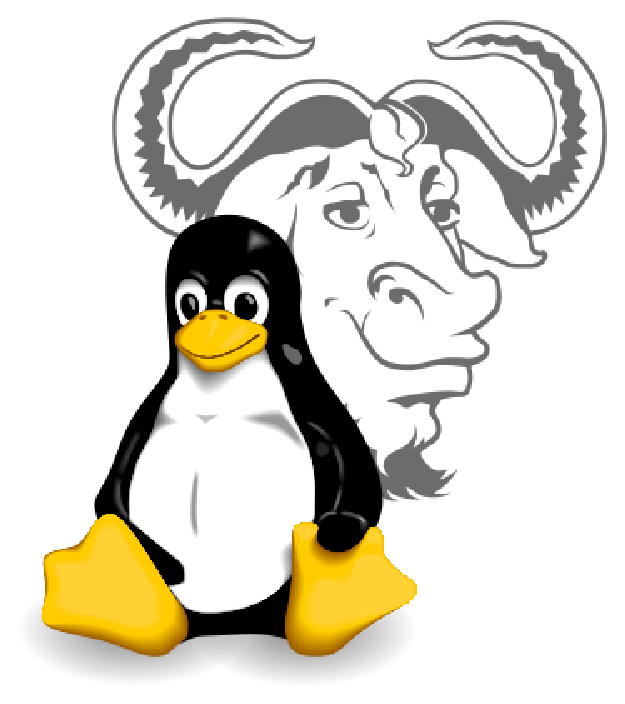
\includegraphics{linux.eps}}
\end{center}
\end{figure}
\end{slide}

\overlays{7}{
\begin{slide}{Co to je?}
\begin{itemize}

\item Operační systém využívající jádro Linux

\fromSlide{2}{
\item Založený na principech unixových systémů
}
\fromSlide{3}{
\item Jeho vývoj začal již v roce 1984 jako součást projektu GNU
}

\fromSlide{4}{
\item Podporuje práci více uživatelů, procesů a je možné jej spouštět na více procesorech
}

\fromSlide{5}{
\item Dokáže spolupracovat s ostatními operačními systémy
}

\fromSlide{6}{
\item Je možné jej používat na různých platformách
}

\fromSlide{7}{
\item Jeho zdrojový kód je veřejně dostupný
}

\end{itemize}
\end{slide}
}

\overlays{7}{
\begin{slide}{Pozoruhodnosti Linuxu}
\begin{itemize}
\item Linux je název jádra vyvinutého 21 letým studentem Linusem Torvaldsem

\fromSlide{2}{
\item Většina jádra je napsaná v čistém jazyce C a některé časti jsou v Assembleru
}

\fromSlide{3}{
\item Oficiální maskot Linuxu je tučňák jménem Tux
}
\fromSlide{4}{
\item Neupravená verze jádra Linuxu se nazývá Vanilla Kernel
}
\fromSlide{5}{
\item Operační systém Android pohánějící dnešní chytré telefony je založen na Linuxu
}
\fromSlide{6}{
\item Celkový počet řádků kódu jádra Linux již překročil 17 milionů
}
\fromSlide{7}{
\item Linux je nejpoužívanějším operačním systémem na superpočítačích a serverech
}
\end{itemize}
\end{slide}
}

\begin{slide}{Linuxové distribuce}
\begin{center}
\begin{tabular}{| l | l |} \hline
\textbf{Distribuce} & \textbf{URL}\\ \hline
Ubuntu & \url{http://www.ubuntu.com/} \\ \hline
Linux Mint & \url{http://www.linuxmint.com/} \\ \hline
Debian & \url{http://www.debian.org/} \\ \hline
Fedora & \url{http://getfedora.org/} \\ \hline
CentOS & \url{http://www.centos.org/} \\ \hline
openSUSE & \url{http://opensuse.org/} \\ \hline
\end{tabular}
\end{center}
\end{slide}

\begin{slide}{Zdroje}
\begin{itemize}
\item \texttt{http://www.tecmint.com/lesser-known-facts-about-gnu-linux/}
\item \texttt{http://www.howtogeek.com/191207/10-of-the-most-popular-linux-distributions-compared/}
\item \texttt{http://www.gnu.org/gnu/linux-and-gnu.html}
\end{itemize}
\end{slide}
\end{document}
